\documentclass{article}
\usepackage[utf8]{inputenc}
\usepackage{graphicx}
\graphicspath{ {images/} }

\title{MicroOS Remote Attestation with TPM and Keylime}
\author{Alberto Planas Dominguez \\ \texttt{aplanas@suse.de}}
\date{October 2021}

\begin{document}

\maketitle

\begin{abstract}
  Trusted Platform Module (TPM) are cryptoprocessors already present
  in any our laptops, desktops, and servers that we bought during the
  last decade.  Frequently overlooked, we are going to explore how
  useful they can be when we have a large number of MicroOS
  installations, and we need to be sure that no one of them has been
  tampered or replaced with a rogue device.
\end{abstract}

\section{Introduction to TPM}
TPM co-processors are not new.  The working group that designed the
specification started in the 90s and produced the first standard in
2009, also the date where the first TPM was commercialized.  Today
they are available in basically any laptop, server, phone or tablet in
the market.

The specification has been driven by the Trusted Computing Group
(TCG)\cite{tcg}, and the last release of describes the TPM version 2.0
of the device\cite{tpm2}.  Because the TPM2 is from 2019, is
reasonable to find devices that still have the version 1.2 or even
1.1b.  Some manufactures support the upgrade of 1.2 to 2.0 via a
firmware update.

TPMs are designed to be very cheap to produce, minimizing the number
of gates and favoring the reuse of some general subsystems.  As a
consequence it is slow for some cryptographic operations, and so TPMs
are useless to speed up some brute force attacks.

Another consequence is that even if the TPM support several
asymmetric-key algorithms, it is recommended to be used to encrypt the
keys of the symmetric-key algorithms that also support, as the former
are much more resource intensive than the later.

Usually TPMs are distributed as an external component attached in the
motherboard, and usually connected via a simple bus connector, like
SPI or I\textsuperscript{2}C.  The last 2.0 specification also support
integrating the TPM inside the CPU.  Also includes different models
like a firmware based TPU (implemented in UEFI) or a virtual TPM
(vTPM) for cloud environments.

Is clear that those different TPM implementations have also different
strengths against physical attacks.  For example, there are documented
hacks\cite{hack} for external TPMs. Must be noted that the
specification leaves to the manufactures all the issues related with
the physical aspect of the security, making room for differentiation.

By the specification, TPMs are not immune to physical attacks.  The
design of the TPMs are focused to defend themselves for software
attacks.  For example, the TPM can generate asymmetric keys and there
is no command that allows the emission of the private part of the key.
Another example is that there is an internal counter that increase for
each fail in providing the correct key, making the next operation
slower (protection against dictionary attacks).

Each TPM have an unique secret asymmetric key pair known as
Endorsement Key (EK), that is injected during the manufacturing
process.  Some manufacturers provisions a certificate for this EK,
that is stored in the NVRAM of the TPM and that can be requested.
This certificate is singed by the manufacturer and can be checked
using the manufacturer public key.  This validation process is key to
set the TPM as a root of trust later on.

\section{Goals of the TPM}
Despite their inexpensiveness, TPM are complex devices that support a
wide range of features.  The last specification make the TPMs
independent of the algorithms used for encryption (RSA and ECC
typically) or cryptographic hashes, deprecating some of them like SHA1
and supporting the implementation of new ones without the requirement
of an update of the specification.  Also now requires the presence on
a non-volatile amount or RAM, that can be useful to persist keys that
would be required very early in the boot process.

\subsection{Identification of devices}
As mentioned, inside each TPM there is a private key put there by the
manufacturer, known as endorsement key (EK).  This key cannot be used
directly, but is used during the generation of secondary keys known as
attestation identity keys (AIK or AK) on demand.

Those secondary keys are associated with the user of the device, and
can be used later to identify the machine inside the network.  Some of
those keys can be generated with the intention of later being migrated
to a different device (note that this kind on keys cannot not be used
for certain operations).

A VPN connection or a SSH session, for example, can be configured to
take this key into consideration during the user login.

\subsection{Key generation}
TPM also provide features to internally generate keys in a secure way.
TPM have a random number generator with some expected quality.

This key can be stored internally, and configured to not be exported
outside of the device.

Those keys are available to the user to, for example, encrypt a file,
volume or full disk if they are stored in the NVRAM.

\subsection{Secure storage of keys}
The new specification requires the presence of some amount of NVRAM,
that can be used to store persistent keys, or keys that need to be
available early in the boot sequence.

Eventually the storage will run out.  With the TPM we can generate a
key pair (the private key will never be communicated to the user) and
the public part will be used to encrypt those other keys stored in the
NVRAM.  The TPM will binary serialize the result in a blob that can be
safely stored on disk.  This blob can later be imported back to the
same TPM if is still valid the private part of the key.

With this mechanism we can generate multiple keys with different
access levels or uses.  As commented before those keys can be
associated to the different users of the device without revealing any
information that can identify them.

\subsection{Random number generator}
As commented there, is also an internal random number generator (RNG)
that can be used internally to generate keys, or externally to feed
user or systems demands.

The implementation details for this RNG are delegated to the
manufacturer, but the specification recommend the usage of entropy
sources like noise or clock variations, among others.  This is later
used feed an internal state-machine that mix it with an one-way
function to generate the next random number.

The random numbers can later be used for seeding the operative
system's own RNG or creating nonces for security protocols, besides
the aforementioned key generation process.

\subsection{NVRAM storage}
The NVRAM available in the TPMs have restricted access-control
properties that can control who can read or who can write from it.

Beside storing keys required during the boot process (for full disk
decryption for example), this memory can be used to store a
representation of the expected state of the machine, in a similar way
that has been done with Secure Boot.

\subsection{Device health attestation}
If something, TPMs were originally designed for the purpose of
detecting alterations in the system, and making very difficult to hide
them to the attacker.

Internally the TPM have 24 platform configuration registers (PCR).
Actually, there is a full set of 24 register for each cryptographic
hash that is supported.  Those registers can be read by the user via
the \emph{quote} operation.  This operation will dump the values of
(maybe a subset) the PCRs in a sort of report that is also signed
internally using a private key stored in the TPM.  The user can
validate this signature to verify that those values are reported
directly from the TPM.

Those register are cleared during each reset cycle (or under demand)
to a good known value. This value is usually zero (\texttt{0x00...0})
but some register can be initialized to \texttt{0x11...1}.

PCRs cannot be directly written, but only updated with an operation
known as \emph{extend}.  Extending a register (see figure
\ref{fig:extend}) is appending the new value that we want to store
with the current value of the register, and storing back the result of
a hash function to the extended value:

\[ PCR <- Hash(PCR || Value) \]

\begin{figure}[h]
  \centering
  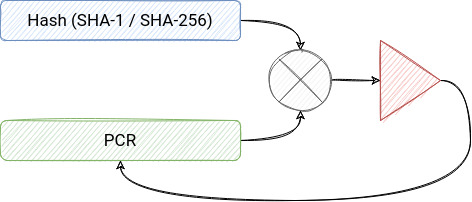
\includegraphics[width=0.75\textwidth]{extend}
  \caption{Extend operation}
  \label{fig:extend}
\end{figure}

With those three operations (\emph{reset}, \emph{quote} and
\emph{extension}) we can describe a safe process (cannot be tampered)
to measure the state of the system.

When the machine is turned on it can check that the TPM is available,
and if so it \emph{reset} the PCR values into a good known state.
This stage, before delegating the execution to the next stage in the
boot chain, will read a segment of this next stage program and
calculate a hash.  This value will be used to \emph{extend} one of the
PCR to store the measure.  After that we can load and jump to the next
stage, that will itself measure the subsequent stage (extending the
same or a different PCR register).

For example PCR0 and PCR1 are extended when measuring the code and
parameters of UEFI.  PCR4 is used for when measuring the boot manager,
and PCR5 for the partition tables.

This process is known as \emph{measured boot}.

For each measurement and extension an event is registered in memory.
First will be stored in some memory area allocated by the UEFI
firmware, and later will be copied to other memory area by the kernel,
that will expose it via the security file system.

An event will register the value that will be used for the extension,
the PCR extended, the kind of event (what has been measured), and some
other data that can be used for later evaluations, like some key
signatures or plain dumps of some memory segments.

A remote agent can request a \emph{quote} (current values of the PCRs,
signed by the TPM) and compare it with the expected values for this
machine.

This process is known a \emph{remote attestation}.

This strategy can be proven to be safe. If an attacker knows the
expected value of a PCR and change some code that belong to the boot
chain, it cannot calculate a value such that an extension with the
current PCR value will produce the expected result.

Also if it try to modify the quote generated by the TPM, it will
invalidate its signature.  Clearing the TPM status will reset the PCR
values and invalidate the attestation keys used for the quote
signature.  Finally, the usage of a nonce when requesting a quote will
also invalidate repetition attacks.

In this process, the only required assumption is the trust in the TPM.

\subsection{Notes about privacy}
One frequent source of concern about the TPMs are related about
privacy and user rights.  TPMs are designed with privacy in mind.  For
example, must be noted that TPMs does not have any access to the
external system, like the memory or the CPU, so are useless to
directly restrict how the machine could be used.

In a similar way, the separation of EK and AIK (and use of certain
protocols) are there to have a mechanism that can validate if a key
has been generated by a TPM, without knowing anything about the TPM
nor the user.

Also, leaking the PCR values shows no information about the device
itself, nor the status.

\section{The TPM Software Stack}
One last comment about the TPM is how are expected to be interacted
with.  The TCG specify for TPM 2.0 a set of APIs, that conform the
TPM2 Software Stack (TSS).  There is currently an open source (BSD-2)
reference implementation published in \emph{github}\cite{tss}.

\begin{figure}[h]
  \centering
  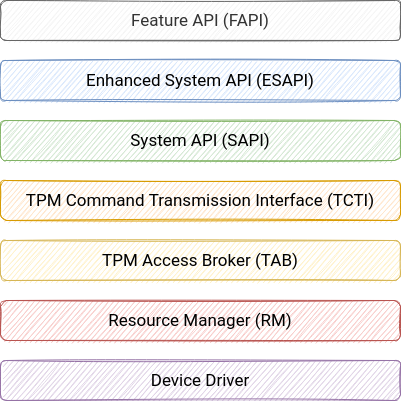
\includegraphics[width=0.75\textwidth]{TPMAPI}
  \caption{TPM2 Software Stack}
  \label{fig:tpmapi}
\end{figure}

In figure \ref{fig:tpmapi} we can identify seven layers for the TSS.

The Feature API (FAPI) is the higher level API for programming TPMs,
and is the one that should be used most of the time as is designed to
simplify the TPM programming as much as possible.

The Enhanced System API (ESAPI) is a direct mapping of the TPM native
commands, but with some helpers like for example session management.
This library have dependencies for other cryptography libraries, and
will allocate memory so is not suitable for very constrains
environments.

The System API (SAPI) is again a mapping of the TPM commands, but this
time without any external dependency nor memory allocation.  Is the
user of the API the one that need to provide the crypto functions.  Is
a library suitable for environment with higher constrains and where a
full control is required.

The TCG specify how we can send commands to the TPM, and how the data
that will be send and received should be serialized.  There are big C
\texttt{struct}s and \texttt{enum}s declared in a headers file.  Some
of the fields are required by some commands, but useless for others.

Because can be expected that some bus communications are slow, the TCG
specify how to identify per command the useless fields, and drop them
to speed up the data transmission.  The TPM Command Transmission
Interface (TCTI) takes care of this type of data serialization, and is
also responsible of sending the commands directly to the TPM.  If we
have a TPM simulator, for example, this component of the stack can be
switched with another library that can communicate to it via the
correct channel (like a socket).

TPM does not support concurrent access from different processes.  The
TPM Access Broker (TAB) takes care of saving the state of the TPM
externally when the TPM needs to attend a different process, and make
like if the full TPM belong to this process.

In a very similar way, because the TPM have a limit of the number of
keys that can store, it should need of the Resource Manager (RM) to
extract encrypted blobs from the TPM that contain the current keys, to
make room to store new ones.

In the Linux kernel those two components (TAB and RM) are also
implement and exposed via a device driver, named \texttt{/dev/tpmr0}.
This is mostly making the \texttt{tpm2-abrmd} service (that implement
the resource manager in TSS), kind of deprecated.

Alternatively the Linux kernel expose the device driver for the TPM in
\texttt{/dev/tpm}, in case that we need to send direct commands.

\subsection{The secret API}
The same group that developed the reference TSS have also the
\emph{tpm2-tools} project.  This is a big collection of command line
tools to interact with the TPM. Well, actually there are only two
binaries: \texttt{tpm2} and \texttt{tss2}, and using soft-links a-la
\emph{busybox} we have access to almost 140 tools and commands.

Initially designed to be used as a base to explore and learn how to
use the TPM, it is also a good approach to develop prototypes and PoC.
For example, the documentation have a very nice example of how to
implement a remote attestation tool using only those CLI
tools\cite{tpm2toolsra}.

In fact, Keylime (a remote attestation tool written in Python) is
using \emph{tpm2-tools} to interact with the TPM.

Sadly, this tool-set substantially changes between versions.  We are
currently in v5.11 and older versions are very different and
incompatible, and it is easy to find outdated documentation.

\section{Keylime}
Keylime\cite{keylime} is an Apache-2.0 project designed to do remote
attestation with the TPM, that is fully integrated with MicroOS.

In Keylime (see figure \ref{fig:keylimearch}) there are three main
components: the \emph{verifier}, the \emph{registrar} and the
\emph{agent}.

\begin{figure}[h]
  \centering
  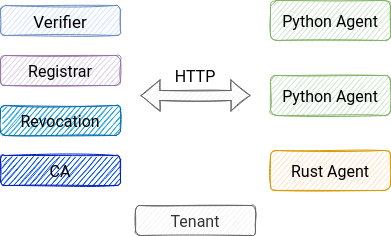
\includegraphics[width=0.75\textwidth]{keylimearch}
  \caption{Keylime Architecture}
  \label{fig:keylimearch}
\end{figure}

The \emph{agent} is a small and light service running in the nodes of
our network.  This service is the one that communicate with the TPM to
request the quote and read the event log published by the kernel, and
send them to the \emph{verifier}.

The \emph{verifier} is the service that will validate the signatures
and the information sent from the different \emph{agents} and,
effectively, validating the state of the remote nodes.

The \emph{registrar} is a service that register all the agent
information (host name, address and certificates, including the TPM
public key of the vendors).

The \emph{tenant} is the name of the CLI tool that we need to use to
add, remove, update or list the different nodes in the network.

All the communication is done via HTTP, but some events are
communicated via \texttt{0mq} sockets.  The HTTP information travels
in clear form, as all the secrets are encrypted and backed up by the
TPM.

\subsection{Keylime features}
The main goal of Keylime is performing the remote attestation of the
measured boot and runtime execution (if IMA/EVM subsystem is
activated) in the node where the agent is running.

We can specify a list of expected PCR values for each agent.  The
\emph{verifier} will request a quote and a copy of the event log to
the \emph{agent}.  The \emph{verifier} then will validate that all the
signatures comes from the respective TPM, and will transverse the
event log to re-do all the calculations of the PCRs, and compare them
with the current values listed in the quote report and the expected
values for them.

Golden values for PCRs are fragile.  An update of one of the
components will make the final expected new value for the PCR very
hard to predict, as we should control all the elements that has been
measured in the system.  In a real world scenario we know the expected
hashes for some of the components, like the UEFI, boot loader, kernel,
kernel command line and maybe the \emph{initrd}.

With Keylime we can prepare Python scripts that can inspect the event
log, and extract from there transient PCR values, extension values,
signatures, or hashes.  Using a set of test combinators, the user can
compare them with some provided referential state.  Keylime provide
those combinators, and a mechanism to register those scripts in the
\emph{verifier}.

If IMA/EVM is activated in the nodes, the \emph{verifier} can also
request the ASCII log that register all the hashes of the executed (or
accessed, depending on the policy in place) files since the
activation.  This list will also include the files from the
\emph{initrd} if the IMA has been activated early (via the kernel
command line, for example).  The \emph{agent} will also send a quote
of the TPM that will include the PCR10, that is expanded each time
that the ASCII log is updated.

If we provide a ``whitelist'' of good hashes (and optionally an
``excludelist'' for the ignored ones), the \emph{verifier} can check
if any of the accessed files in the system has been changed.

Keylime provides a mechanism for delivering an encrypted payload to
the agents.  Basically is a \texttt{zip} file that contains the
payload and a shell script that will be executed on the agent.  This
file is decoded and decompressed in a security file system mounted and
controlled by the agent.

Additionally there is a plugin-based revocation framework.  When the
\emph{verifier} detect a non authorized change in the system, it will
emit a revocation certificate, and an event will be delivered via
\texttt{0mq} that will be received by all the agents.  An
user-provided Python code (delivered previously via the encrypted
payload) will be executed in all the nodes, with the information about
the type of event, and the nodes affected by it.  We can use this code
to execute the commands that will prevent to the (maybe) compromised
note to have access to the resources of the network.

The communication between the Keylime service is following a versioned
RESTfull API.  This allows, for example, the presence of two different
implementation for the \emph{agent} service, one written in Python and
a newer one in Rust.

Finally, in MicroOS we updated the YaST system roles to include two
new roles.  One that will deploy the control plane of Keylime (the
\emph{verifier} and \emph{registrar}) and the other for the
\emph{agents}.

We deployed a patched version of Keylime, with an almost ready
configuration file (ideally the only change is pointing to the
\emph{verifier} IP address in the \emph{agent} nodes) and a revocation
service based on \emph{CFSSL} instead on the default \emph{openSSL},
that is not fully supported.

\subsection{Using Keylime}
We published some documentation about the integration of Keylime with
MicroOS\cite{microosra}, including how it is expected to be
configured, how to enable features based on IMA, how to create the
white list, the payload, and a example of usage.  In this section we
are going to have a short version of the Keylime demonstration
described in the MicroOS documentation, but can be useful to present
here some of the steps.

In the demo we prepared three nodes, one deployed with the
\emph{verifier} system role, and the others two with the \emph{agent}
system role.  On one of them we enabled IMA updating the default
kernel command line and rebooting later.

We also prepared in this node a list of good hashes, using a manual
approach, that was later copied into the \emph{verifier}.  Sadly, this
was required for two reasons:

\begin{itemize}
\item Our \emph{RPM} packages are not currently deploying the IMA
  hashes in the extended attributes
\item Downloading the \emph{RPM} package from the repository can be
  useful, but will not contain the contents of the \emph{initrd}, and
  some configuration files created by the package \emph{scriptlets}.
\end{itemize}

Instead of specifying a list of golden values for the PCRs (and using
the \texttt{--tpm\_policy} parameter to indicate the list of possible
values; see the MicroOS Remote Attestation documentation for more
information), we decided to simplify the demo declaring an empty
reference state.  This will fetch the event log and re-calculate the
final values of the PCR.  For more complex policy, the example policy
can now be used\cite{examplepolicy}.

A payload was created to include some \emph{ssh} keys, that the
payload script (\texttt{autorun.sh}) will put in place on each node to
enable passwordless access.

We also included a Python script that will be executed when a
revocation event is communicated (\texttt{local\_action\_rm\_ssh.py}).
This script have two sections, one will be executed in the node that
has been revoked, that will remove the \emph{ssh} keys from the
system.  We should not trust this section, as we need to consider this
node compromised.  The second section will be executed in the rest of
the nodes, and in this example will call \texttt{iptables} to force
the isolation of the affected node.

With this in place, we can register the nodes in Keylime.

\begin{verbatim}
keylime_tenant -v verifier.suse.de \
  -t agent.suse.de \
  -u AGENT-UUID \
  --cert default \
  --include payload \
  --allowlist ./allowlist.txt \
  --exclude ./exclude.txt \
  --mb_refstate mb-refstate.json \
  -c add
\end{verbatim}

This will instruct the \emph{verifier} to frequently request the
measured boot information, together with the list of hashes of the
files that the node has opened, all this certified by the local TPM.
This information is validated against the PCR values from the quote
(also requested together with a nonce).

After the first validation, the payload (already encrypted and
deployed), would be decrypted and decompressed by the \emph{agent},
and the auto run script executed in the Keylime context.  This will
move \emph{ssh} the keys in to the expected place.

Now, any change in the \emph{agent} node can be detected by the
\emph{verifier}. If this happens, a revocation event will be send to
all the nodes, that will trigger the execution of all the local action
scripts delivered in the payload.  In this case the local action will
remove the \emph{ssh} keys in the modified node, and fence the rest of
the them against the hacked node.

\section{Conclusion and future work}
Keylime is already integrated in MicroOS, but there are areas that can
be improved.

We think that the main pain point is the white-list generation of IMA
hashes.  This is a manual process documented in the MicroOS Remote
Attestation portal.  Ideally the IMA hashes should be available inside
the RPM, and written in the file extended attributes during the
installation.  This can already be done by \emph{rpm-plugin-ima}, but
the OBS sign module do not support this feature.

There is a comprehensive documentation of IMA/EVM in
openSUSE\cite{ima}, that shows that there are other issues that can
affect SELinux and systemd.

If we manage to resolve those issues and deliver the IMA hashes in the
RPM, signed by SUSE, we can start thinking about different mechanism
that will extract this information without accessing the different
nodes where those packages will be installed.

Keylime itself is not an easy tool to use.  Any mistake in the
parameters will throw an exception, instead of writing a descriptive
error message.  There is some inconsistency in the parameter names,
and some areas like the tests combinators that would require some
formal approximation to be generally useful.

\begin{thebibliography}{9}
\bibitem{tcg}
  Trusted Computing Group. \emph{https://trustedcomputinggroup.org}

\bibitem{tpm2}
  TPM 2.0 Library. \emph{https://trustedcomputinggroup.org/resource/tpm-library-specification/}

\bibitem{hack}
  From Stolen Laptop to Inside the Company Network. \emph{https://dolosgroup.io/blog/2021/7/9/from-stolen-laptop-to-inside-the-company-network}

\bibitem{tss}
  TPM2 Software Stack. \emph{https://github.com/tpm2-software/tpm2-tss}

\bibitem{tpm2toolsra}
  Remote Attestation with tpm2-tools. \emph{https://tpm2-software.github.io/2020/06/12/Remote-Attestation-With-tpm2-tools.html}

\bibitem{keylime}
  Keylime. \emph{https://keylime.dev}

\bibitem{examplepolicy}
  Keylime example policy. \emph{https://github.com/keylime/keylime/blob/master/keylime/elchecking/example.py}

\bibitem{microosra}
  MicroOS Remote Attestation. \emph{https://en.opensuse.org/Portal:MicroOS/RemoteAttestation}

\bibitem{apgtpm2}
  Will Arthur, David Challener (2015) \emph{A Practical Guide to TPM2.0}, Springer Nature.

\bibitem{trustedcomp}
  Aries Siegal Lectures. \emph{https://opensecuritytraining.info/IntroToTrustedComputing.html}

\bibitem{ima}
  openSUSE IMA/EVM. \emph{https://en.opensuse.org/SDB:Ima\_evm}
\end{thebibliography}

\end{document}
